\documentclass[conference, letterpaper]{IEEEtran}
%\documentclass[a4paper]{article}

\ifCLASSINFOpdf \else \fi

\usepackage[pass]{geometry} \usepackage{tabularx} \usepackage{graphicx}
\usepackage{amssymb} \usepackage{algorithm} \usepackage{algorithmic}
\usepackage{amsmath} \usepackage{booktabs} \usepackage{caption}

\usepackage{cite} \usepackage[numbers,sort&compress]{natbib}
\captionsetup[table]{position=top,labelfont={sc},textfont={sl}}

\renewcommand{\thetable}{\Roman {table}}

\title{ Use of Model Predictive Control (MPC) for Rocket Altitude Correction }

\author{ \IEEEauthorblockN{Nikhil Peri, Anthony Lin, Manit Ginoya, Paul Buzuloiu } \
\IEEEauthorblockA{uOttawa Rocketry Team \\ \{nperi104, alin102
mgino015, pbuzu025\}@uottawa.ca} }

\begin{document}
\maketitle
\begin{abstract}
\end{abstract}

Keywords—Model Predictive Control, Aerospace.  \section{Introduction}

Rockets unlike other aircraft have high speed and dynamic flights, as a result
rocket control systems have to be extremely responsive and precise. Classical
control systems based on observed sensor feedback would not be able to meet the
demands of rocket flight since the latency between plant actuation affecting the
the physical world and detecting that change through sensor observations is too
slow for such dynamic flight environments. Model Predictive Control (MPC) solves
these problems by introducing state estimation.  This process involves maintaining
a kinetic model of the actuators we are using for altitude control, in this case
is a drag model for a drag inducing airbrake system. Using this model we can predict
the effect of actuation on the target altitude. #TODO finish this with the speficic MPC schema that we are using

\section{System States}
In both classical and MPC design it is important to first outline all the system states.
For most kinetic systems these are the acceleration, velocity and position of the object
being controlled for each axis x, y, z in the state space representation below

\begin{equation}
\begin{bmatrix}\dot{p_x}\\\dot{v_x}\\\dot{a_x}\end{bmatrix}=
\begin{bmatrix}\0 \ 1\ 0\\0 \ 0\ 1\\0\0\0\end{bmatrix}
\begin{bmatrix}p_x\\v_x\\a_x\end{bmatrix}
\end{equation}

These vectors need to be projected on a single reference frame, and for the purposes of calculating
rocket trajectory after lift-off and maximum altitude above the ground it makes the most sense to
use the earth as a reference frame.

We also have the additional rotation around each of the specified axis commonly referred to as
pitch roll and yaw

\begin{figure}[H]
\centering
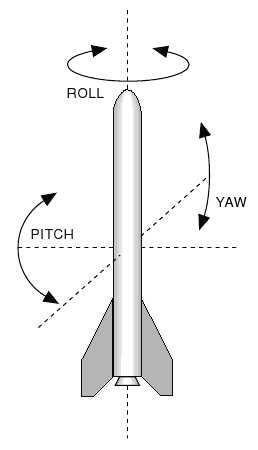
\includegraphics[scale=0.30]{./pitch_roll_yaw}
\caption{Rocket Axis of Rotation}
\label{fig:pitch_roll_yaw}
\end{figure}

For simplicity we can omit the roll since it does not contribute to the heading of the rocket in flight.
We can then apply the following reference frame transformation to convert the acceleration experienced
by the rocket to the acceleration it is experiencing with reference to the earth frame using the Euclidian Matrix
\ref(mallick_2016)

\begin{equation}
  \begin{bmatrix}\ a_x\\\ a_y\\\ a_z\end{bmatrix}=
  \begin{bmatrix}
    cos(\theta_x) & sin(\theta_x)sin(\theta_y) & sin(\theta_x)cos(\theta_y) \\
    0 & cos(\theta_y) & -sin(\theta_y) \\
    sin(\theta_y) & cos(\theta_x)sin(\theta_y) & cos(\theta_x)cos(\theta_y) \\
  \end{bmatrix}
  \begin{bmatrix} a'_x \\ a'_y \\ a'_z \end{bmatrix}
\end{equation}

Where \theta_x is the yaw and \theta_y is the pitch of the rocket. These form the state space for our rocket
system and most 3D kinetic systems

\section{Airbrake Model}
The Airbrake is our primary control surface, it is actuated by a servo that deploys
set of fins out of streamlined rocket body.  These can be used to increase the drag on
the rocket body as a result reducing the velocity and final altitude of the rocket.

\begin{figure}[H]
\centering
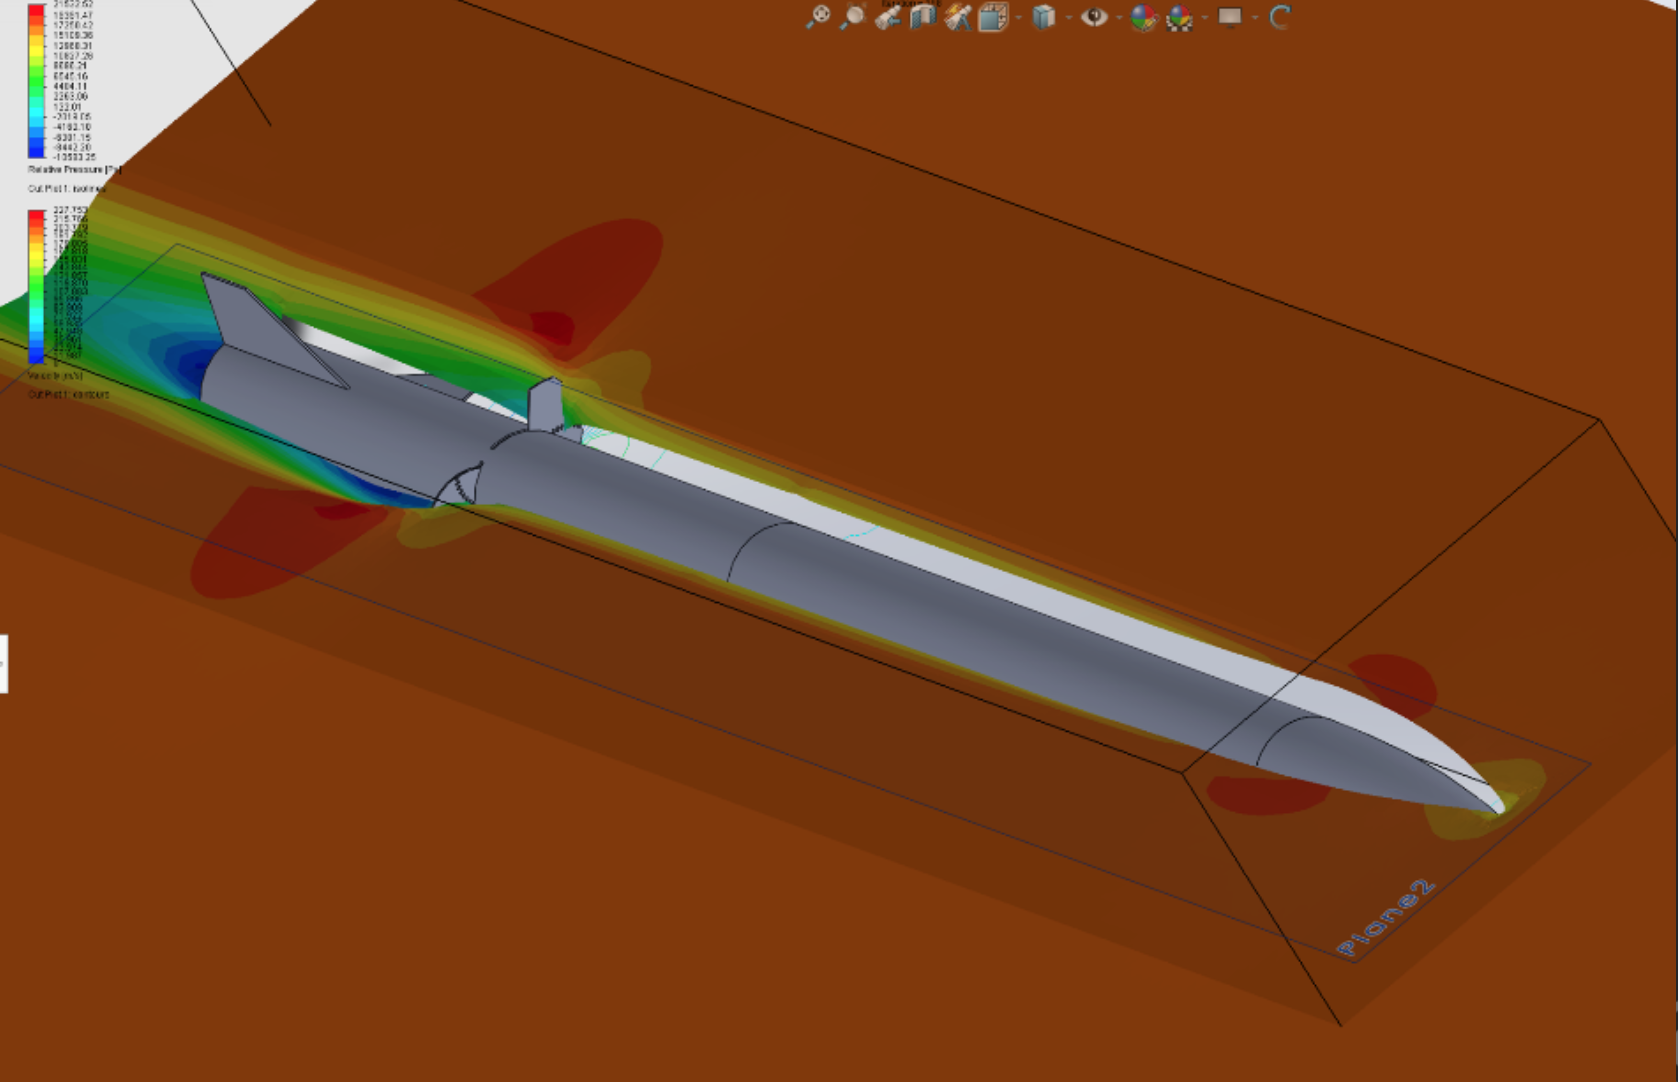
\includegraphics[width=0.45\textwidth]{./airbrake_mechanism}
\caption{Airbrake Mechanism}
\label{fig:airbrake_mechanism}
\end{figure}

The drag force is a function of the surface area and relative velocity as seen below

\begin{equation}
  F_{drag}(V, A)=\frac{1}{2}C_dV^2A\rho
\end{equation}

In order to characterize this system we must determine the drag coefficient of the rocket
during airbrake deployment.  Due to the similicity of the Airbrake we can use a basic
model for the experimentally determined drag of a flat plate which is \ref(nasa)

\begin{equation}
  C_d=1.28
\end{equation}

But since this drag model will be used to predict final state
\section{Model Predictive Control}

The complexity of rocket flight partially arises from the numerous states
required to fully define an entire set of dynamics. These states include
acceleration, velocity, position, orientation, angular speed and angular
acceleration of the rocket in all three spatial dimensions. Additionally,
the states related to the actuators (in this case, the servo motor controlling
the airbrakes) must also be considered. Desiging a classical controller or even
a digitally implmented classicial controller would bring along several
inconveniences; for this reason, a model predictive controller was considered
and implemented.

The major concept of model predictive control is to maintain a real time
simulation; This simulation's role is to produce a prediction of future system
states using feedback from sensors and the system's current states. For the case
of achiving a particular target altitude by deploying airbrakes, the MPC will
produce a predicted final altitude
every control loop. Using this predicted final altitude, the error between the
predicted final altitude and the desired final altitude will be calculated. The
final part of the MPC process is to map the calculated error to a specific
(whether heuristic or deterministic) control signal that will be sent to the
airbrake actuator.

Figure \ref{fig:MPC_diagram} is the fully defined control system diagram
corresponding to the description provided above. Running through the control
schema yeilds the following sequence of events: sensors are read, filtered and
fused, states are estimated, trajectory is predicted, final altitude error is
determined, control signal is generated, signal is sent to actuator driver,
actuation occurs which affects rocket flight.

\begin{figure}[H]
\centering
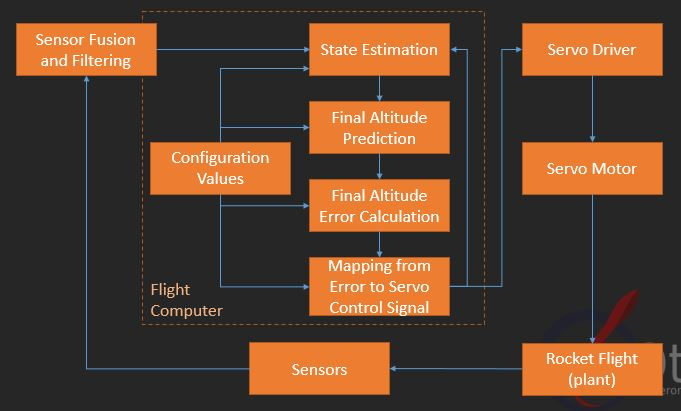
\includegraphics[width=0.45\textwidth]{./MPC_diagram}
\caption{Overall Control Diagram of airbrake system}
\label{fig:MPC_diagram}
\end{figure}

When comparing figure \ref{fig:MPC_diagram} to a
typical control systems diagram, the input to the system seems to be missing;
This input (the desired final altitude) is merely hidden away as a part of the
digitally implemented configuration values. Some important inferences of the
presented control diagram include understanding that the configuration values
include all phycial rocket parameters, as well as the desired final altitude.
Therefore, the presented figure is related more to the physcial implementation
than to control theory notation.

\section{Imeplementation}

Here, each block residing withing the flight computer as shown in
the diagram presented in figure \ref{fig:MPC_diagram} is
defined further to provide insight into the implementation of this
system.

\subsection{Sensor Fusion}

In order to achieve accurate state estimation, which is an essential functional
component of the control schema, certain feedback values are required in a
non-inertial frame. However the sensors on board the rocket can only measure
quantities in an inertial frame. Therefore, the sensor fusion block is necessary
to not only filter sensor values but also to acquire accurate feedback values in
a non-inertial frame.

To determine what types of filtering and fusion are required, it is helpful to
first determine a set of sensors that will be used. Figure \ref{fig:sensors}
dipicts the three main modules of sensors being used. They are, shown left to right,
Yost Labs 3 space LX Embedded IMU, Adafruit MTK3339 GPS and the MPL3115A2 altimeter.

\begin{figure}[H]
\centering
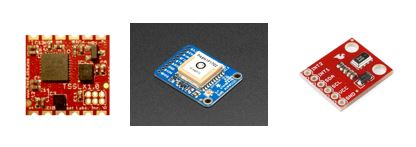
\includegraphics[width=0.45\textwidth]{./sensors}
\caption{Image of Sensors Used for System Implementation}
\label{fig:sensors}
\end{figure}

These sensors were chosen to help minimize the amount of self developed fusion and
filtering. The Yost Labs 3 space LX Embedded IMU has nine degrees of freedom and
provides filtered, three dimensional acceleration, speed and position in a
non-inertial frame (via proprietary, low level embedded algorithms). Using the data
from this sensor module, all required feedback values for state estimation can be
satisfied. However to make the state estimation as accurate as possible, the
stand alone GPS and altimeter modules will be used to correct IMU drift and
perform self-checking.

\subsection{State Estimation}

The state estimation block uses the feedback values from sensors (after filtering and fusion)
and the previous states of the system to calculate the current state of the system.
Since the feedback values already provide measured acceleration, speed and position
in a non-inertial frame, they can be used directly to update the states of the system.
However,


\subsection{Final Altitude Prediction}

\subsection{Final Altitude Error Calculation}

\subsection{Mapping from Error to Control Signal}

\section{Conclusion}

In this brief, an implementation of model predictive control is presented for a
custom airbrake system to be deployed on a sounding rocket. The convenience of
using MPC for this specific application is shown. Furthermore, and with some
modification, it is shown that the implemented MPC can be deployed on cheap electrical
hardware.

\section{Acknowledgement}

The authors would like to thank the University of Ottawa for continued support of the
rocketry team. Additionally, specific thankfulness is issued to professor Habash and
the teaching assistants of the ELG 4157 course.

\bibliographystyle{unsrt}
\bibliography{references}
\end{document}
